\section{2-Körperproblem -- Kepler Gesetze}
\paragraph{Skizze:}
\begin{center}
    \tdplotsetrotatedcoords{0}{0}{90}
    \begin{tikzpicture}[scale=2,tdplot_rotated_coords]
        \coordinate (O) at (0,0,0);
        \coordinate [label=left:{$m_1$}] (m1) at (-1,1,-0.2);
        \coordinate [label=right:{$m_2$}] (m2) at (1,1.2,0.4);
        \coordinate (S) at (0,1.1,0.1);

        \draw [thick,->] (O) -- (1.2,0,0) node [anchor=north west] {$x$};
        \draw [thick,->] (O) -- (0,1.2,0) node [anchor=south west] {$y$};
        \draw [thick,->] (O) -- (0,0,1.2) node [anchor=south] {$z$};

        \draw [->] (O) -- (m1) node [pos=0.5,anchor=north east] {$\vec r_1$};
        \draw [->] (O) -- (m2) node [pos=0.5,anchor=north west] {$\vec r_2$};
        \draw [->] (m1) -- (m2) node [pos=0.5, anchor=south] {$\vec r$};
        \draw [->] (O) -- (S) node [pos=0.5, anchor=east] {$R$};
    \end{tikzpicture}
\end{center}

\paragraph{DGL}
\begin{align*}
    m_1 \vec r_1 + m_2 \vec r_2 = \frac{d^2}{dt^2} (m_1 \vec r_1 + m_2 \vec r_2) &= \vec 0 \tag*{$| \dfrac{m}{m}$} \\
    \Rightarrow m \frac{d^2}{dt^2} \underbrace{\left(\frac{m_1\vec r_1 + m_2 \vec r_2}{m}\right)}_{\mathclap{= \vec R = \frac{\vec C_2}{m} \text{für $\vec C_1 = \vec P_{\mathrm{ges}}$}}} = \vec 0 \Leftrightarrow m \ddot{\vec{R}} &= \vec 0
\end{align*}
\[ \boxed{m\ddot{\vec{R}} = \vec 0} \]
\framebox{$\Rightarrow$ Referezsystem bzgl. Massenschwerpunkt muss ein Inertialsystem sein}

$\Rightarrow$ \textbf{Wahl:} Koordinatenursprung im Schwerpunkt $\Leftrightarrow \vec{R} = \vec 0$

\subsection{Koordinatentransformation}
\begin{center}
    \begin{minipage}[h]{.5\textwidth}
        \centering
        \tdplotsetrotatedcoords{0}{0}{90}
        \begin{tikzpicture}[scale=2,tdplot_rotated_coords]
            \coordinate (O) at (0,0,0);
            \coordinate [label=left:{$m_1$}] (m1) at (-1,-0.1,-0.3);
            \coordinate [label=right:{$m_2$}] (m2) at (1,0.1,0.3);
            \coordinate (S) at (0,0,0);

            \draw [thick,->] (O) -- (1.2,0,0) node [anchor=north west] {$x$};
            \draw [thick,->] (O) -- (0,1.2,0) node [anchor=south west] {$y$};
            \draw [thick,->] (O) -- (0,0,1.2) node [anchor=south] {$z$};

            \draw [->] (O) -- (m1) node [pos=0.5,anchor=south] {$\vec r_{S1}$};
            \draw [->] (O) -- (m2) node [pos=0.5,anchor=south] {$\vec r_{S2}$};
            \draw [->] ([yshift=-1pt]m1) -- ([yshift=-1pt]m2) node [pos=0.5, anchor=north] {$\vec r_S$};
            \draw [->] (O) -- (S) node [pos=0.5, anchor=south] {$R$};
        \end{tikzpicture}
    \end{minipage}
    \begin{minipage}[h]{.4\textwidth}
        \begin{align*}
            \vec R_S &= \frac{m_1 \vec r_{S1} + m_2 \vec r_{S2}}{m} = \vec 0 \\
            \vec r_S &= \vec r_{S2} - \vec r_{S1} \\
            m &= m_1 + m_2
        \end{align*}
    \end{minipage}
\end{center}

\begin{enumerate}[i)]
    \item \begin{align*}
            \frac{m_1}{m} \vec r_{S1} + \frac{m_2}{m} \vec r_{S2} &= \vec 0 \\
            \Rightarrow \vec r_{S1} \underset{= 1}{\left(\cancel{\frac{m_1 + m_2}{m}}\right)} &= - \vec r_S \frac{m_2}{m} \\
                                                                                              &\Rightarrow \boxed{\vec r_{S1} = - \frac{m_2}{m} \vec r_S}
        \end{align*}
    \item Analog $\boxed{ \vec r_{S2} = \dfrac{m_1}{m} \vec r_S }$
\end{enumerate}

\begin{definition}
    Reduzierte Masse:
    \[ \boxed{\mu := \frac{m_1 m_2}{m}} \]
\end{definition}

$\Rightarrow$ \textbf{Vektoren im Schwerpunktsystem:}
\[ \vec r_{S1} = - \frac{\mu}{m_1} \vec r_S; \qquad \vec r_{S2} = \frac{\mu}{m_2} \vec r_S\]

\subsection{Eigenschaften im Schwerpunktsystem}
\subsubsection{Energie des 2-Körperproblems}
\begin{align*}
    E &= E_{\mathrm{kin}} + E_{\mathrm{pot}} \\
      &= \sum\limits_{i=1}^2 \frac{m_i}{2} \dot r_i^2 - \frac{G m_1 m_2}{r} \\
    E &\mathrel{\overset{\mathclap{
        \begin{matrix}
            \text{Schwerpunktsystem} \\
            \downarrow
        \end{matrix}
        }}=} \sum\limits_{i = 1}^2 \frac{m_i}{2} \dot r_{Si}^2 - \frac{G m_1 m_2}{r_S} \\
      &= \frac{\cancel{m_1}}{2} \left(- \frac{\mu}{\cancel{m_1}}\right) \dot r_S^2 +
         \frac{\cancel{m_2}}{2} \left(- \frac{\mu}{\cancel{m_2}}\right) \dot r_S^2 -
         \frac{G m_1 m_2}{r_S}\\
      &= \frac{\mu^2}{2} \dot r_S^2 \underbrace{\left(\frac{1}{m_1} + \frac{1}{m_2}\right)}_{\mu^{-1}}
         - \frac{G m \mu}{r_S} \\
      &= \boxed{\frac{\mu}{2} \dot r_S^2 - \frac{Gm\mu}{r_S} = E}
\end{align*}

\subsubsection{Interpretation}
\begin{itemize}
    \item Die Energie des System entspricht der $E_{\mathrm{kin}}$ der reduzierten 
          Masse zusammen mit der $E_{\mathrm{pot}}$ der reduzierten Masse,
          die sich um die Gesamtmasse $m$ im Schwerpunkt (angenommen) bewegt.
    \item Abstand $|\vec r_S| = r_S$ zwischen reduzierter und Gesamtmasse
          entspricht dabei dem Abstand zwischen $m_1$ und $m_2$
\end{itemize}

\paragraph{Analog} $\vec L_S$ im Schwerpunktsystem (s. Übungen)

\paragraph{Allgemein} Äquivalentes 1-Körperproblem
\begin{center}
    \begin{minipage}[h]{.5\textwidth}
        \centering
        \tdplotsetrotatedcoords{0}{0}{90}
        \begin{tikzpicture}[scale=2,tdplot_rotated_coords]
            \coordinate (O) at (0,0,0);
            \coordinate [label=right:{$\mu$}] (mu) at (1,0.1,0.3);

            \draw [thick,->] (O) -- (1.2,0,0) node [anchor=north west] {$x$};
            \draw [thick,->] (O) -- (0,1.2,0) node [anchor=south west] {$y$};
            \draw [thick,->] (O) -- (0,0,1.2) node [anchor=south] {$z$};

            \draw [->] (O) -- (mu) node [pos=0.5,anchor=south] {$\vec r_{S}$};
        \end{tikzpicture}
    \end{minipage}
    \begin{minipage}[h]{.4\textwidth}
        \centering
        \tdplotsetrotatedcoords{0}{0}{90}
        \begin{tikzpicture}[scale=2,tdplot_rotated_coords]
            \coordinate [label=below:{$\mathcal M_{\astrosun}$ Sonne}] (m1) at (0,-1,-1);
            \coordinate [label=above:{$m_{\mathrm{Pl}}$ Planet}] (m2) at (0,1,1);

            \draw [->] (m1) -- (m2);
        \end{tikzpicture}
    \end{minipage}
\end{center}

\paragraph{Speziell:}
\[ \boxed{\underset{= m_1}{\mathcal M_{\astrosun}} \gg \underset{= m_2}{m_{\mathrm{Pl}}}} \]

\[ \Rightarrow \left\{ \begin{array}{r@{\ }l}
            m &= \mathcal M_{\astrosun} + m_{\mathrm{Pl}} \approx \mathcal M_{\astrosun} \\
            \mu &= \frac{\cancel{\mathcal M_{\astrosun}} \cdot m_{\mathrm{Pl}}}{\underbrace{(\mathcal M_{\astrosun} + m_{\mathrm{Pl}})}_{\approx \cancel{\mathcal M_{\astrosun}}}} \approx m_{\mathrm{Pl}}
\end{array} \right. \]

Es gilt:
\begin{align*}
    \cancel{\mu} \ddot \vec r_S &= -\frac{Gm\mu \vec r_S}{r_S^3} \tag*{$\left| \begin{array}{r@{\ }l}
        \times \vec L_S &= \vec{\mathbf{const}} \\
               \vec L_S &= \vec r_S \times \mu \dot \vec r_S
    \end{array} \right.$} \\
    \Rightarrow \ddot \vec r_S \times \vec L_S &= - \frac{G m \vec r_S}{r_S^3} \times \vec L_S \\
        &= - \frac{Gm}{r_S^3} \vec r_S \times (\vec r_S \times \mu \dot \vec r_S) \\
        &= - \frac{Gm\mu}{r_S^3} [\vec r_S \underbrace{(\vec r_S \times \dot \vec r_S)}_{?} 
            - \dot \vec r_S \underbrace{\langle\vec r_S, \vec r_S\rangle}_{r_S^2}]
\end{align*}

$bac$-$cab$-Regel:
\[ \vec a \times \vec b \times \vec c = \langle \vec b, \langle \vec a, \vec c\rangle\rangle - \langle\vec c, \langle \vec a, \vec b\rangle\rangle \]

\color{OliveGreen}
\textbf{Nebenrechnung:}
\begin{align*}
    \langle\vec r, \dot\vec r\rangle &= \dot r_S r_S \\
    \frac{d}{dt} \underbrace{\langle \vec r_S, \vec r_S\rangle}_{r_S^2} &= 2 \langle \vec r_S, \dot r_S \rangle \\
    \frac{d}{dt} r_S^2 &= \cancel{2} r_S \dot r_S
\end{align*}
\color{black}

\begin{align*}
    \ddot \vec r_S \times \vec L_S &= - \frac{Gm \mu}{r_S^3} (\vec r_S (r_S \dot r_S) - \dot \vec r_S r_S^2) \tag*{$| \cdot Gm\mu$} \\
    \frac{d}{dt} (\dot \vec r_S \times \vec L_S) &= \ddot \vec r_S \times \vec L_S + \dot \vec r_S \times \underset{=0}{\cancel{\dot{\vec{L}}_S}} \\
    \Rightarrow \frac{d}{dt} \frac{(\dot \vec r_S \times \vec L_S)}{G m \mu} &= \frac{\dot \vec r_S \cancel{r_S^2}}{r_S^{\cancel{3}}} - \vec r_S \frac{\cancel{r_S} \dot r_S}{r_S^{\cancel{3}^2}} =
    \underbrace{\frac{\dot \vec r_S}{r_S} - \frac{\dot r_S}{r_S^2} \vec r_s}_{= ?}
\end{align*}

\color{OliveGreen}
\textbf{Nebenrechnung:}
\[ \frac{d}{dt} \left(\frac{\vec r_S}{r_s}\right) = \frac{\dot \vec r_S}{r_S} - \frac{\vec r_S - \dot r_S}{r_S^2} \]
\color{black}

$\Rightarrow$ \textbf{DGL}:
\[ \frac{d}{dt} \left(\frac{\dot \vec r_S \times \vec L_S}{G m \mu}\right) = \frac{d}{dt} \left(\frac{\vec r_S}{r_S}\right) \tag*{$| \int dt$} \]

\textbf{Lösung:}
\begin{align*}
    \frac{1}{Gm\mu} (\dot\vec r_S \times \vec L_S) &= \frac{\vec r_S}{r_S} + \vec{\textbf{const}} = \frac{\vec r_S}{r_S} + \varepsilon \vec e \tag*{$| \langle\cdot, r_S\rangle$} \\
    \Rightarrow \frac{r_S^2}{r_S} + \varepsilon \underbrace{(\langle \vec e, \vec r_S)}_{\mathclap{= 1 \cdot r_S \cdot \cos \varphi}} &= r_S (1 + \varepsilon \cos \varphi) = \frac{1}{Gm\mu} \underbrace{\langle \vec r_S, \dot \vec r_S \times \vec L_S}_{\text{Spatprodukt}} \\
        &= \frac{1}{Gm\mu} \underbrace{(\vec r_S \times \dot \vec r_S)}_{= \frac{\vec L_S}{\mu}} \cdot \vec L_S =
           \frac{1}{Gm\mu} L_S^2 = \mathbf{const} =: P\\
        &\Rightarrow \boxed{r_S = \frac{P}{1 + \varepsilon \cos \varphi}} \qquad \text{Kegelschnitt (1. \textsc{Kepler}'sches Gesetz)}
\end{align*}

\subsubsection{Kegelschnitt}
\begin{description}
    \item[$\varepsilon:$] Bahnexzentrizität
    \item[$\varphi:$] wahre Anomalie
    \item[$\vec e:$] Einheitsvektor fest in Richtung Perihel
\end{description}

Bahnform ist ein Kegelschnitt in Abhängigkeit von der Energie
\begin{center}
    \begin{tabular}{|r@{:\ }l|l}
        \cline{1-2} $E < 0$ & Ellipse & (gebundenes System) \\
        $E = 0$ & Parabel \\
        $E > 0$ & Hyperbel & (ungebundenes System) \\\cline{1-2}
    \end{tabular}
\end{center}

\paragraph{Parameter der Bahnformen}
\begin{center}
    \begin{tabular}{r|cccc}
                        & \textbf{Kreis}    & \textbf{Ellipse}          & \textbf{Parabel}  & \textbf{Hyperbel} \\\hline
        $\varepsilon$   & 0                 & $0 < \varepsilon < 1$     & 1                 & $\varepsilon > 1$\\
        $P$             & $a$               & $a (1 - \varepsilon^2)$   & $P$               & $a(\varepsilon^2 - 1)$\\
        $a$             & $a$               & $a$                       & ---               & $a$\\
        $b$             & $a$               & $a\sqrt{1 - \varepsilon^ 2}$ & ---            & $a \sqrt{\varepsilon^2-1}$
    \end{tabular}
\end{center}

\paragraph{Drehimpuls für Ellipse}
\begin{align*}
    L_S &= \mu \sqrt{GmP} = \mu \sqrt{Gma(1-\varepsilon^2)} \\
    \lim\limits_{\varepsilon \to 0} L_S &\longrightarrow \max\limits_{\mathclap{\text{(Kreis)}}} & \lim\limits_{\varepsilon \to 1} L_S &\longrightarrow \underset{\mathclap{\text{(Parabel)}}}0
\end{align*}

\paragraph{Skizze} Flächengeschwindigkeit $A$
\begin{center}
    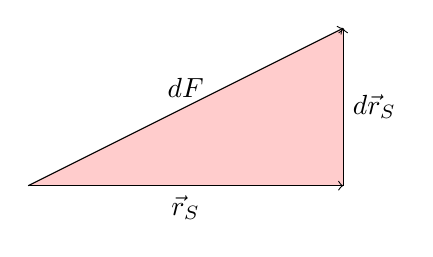
\begin{tikzpicture}[scale=2]
        \coordinate (O) at (0,0);
        \fill[fill=red!20] (O) -- (2,0) -- (2,1);
        \draw[->] (O) -- (2,0) node [pos=0.5,below] {$\vec r_S$};
        \draw[->] (2,0) -- (2,1) node [pos=0.5,right] {$d \vec r_S$};
        \draw[->] (O) -- (2,1) node [pos=0.5,above] {$d F$};
    \end{tikzpicture}
\end{center}

\begin{align*}
    dF &= \frac{1}{2} | \vec r_S \times d \vec r_S | \tag*{$| \cdot dt$} \\
    \Rightarrow \frac{dF}{dt} &= \frac{1}{2} \underbrace{\left| \vec r_S \times \frac{d\vec r_S}{dt}\right|}_{= \frac{|\vec L_S|}{\mu}} = \frac{1}{2\mu} | \vec L_S | = A
\end{align*}

Gesucht: $A = \mathbf{const} \Leftrightarrow \dot A = 0$
\begin{center}
    $\dfrac{d}{dt} = \dfrac{d}{dt} \dfrac{L_S}{2 \mu} = \dfrac{\overset{= 0}{\dot L_S}}{2 \mu} = 0$, wenn Drehimpulserhaltung $\dot{\vec{L}}_S = \vec 0$ \\
    $\Rightarrow \boxed{A = \frac{L_S}{2\mu} = \mathbf{const}}$ (2. \textsc{Kepler}'sches Gesetz)
\end{center}

\paragraph{Betrachte} Fläche der Ellipse $F$

